\section{Waves}

\begin{multicols}{2}


\section*{Introduction to Waves}


\subsection{String Waves}

\begin{center}
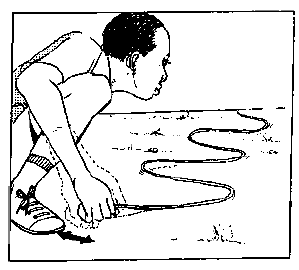
\includegraphics[width=0.4\textwidth]{./img/source/string-waves.png}
\end{center}

\begin{description*}
%\item[Subtopic:]{}
\item[Materials:]{}
\item[Setup:]{}
\item[Procedure:]{}
\item[Hazards:]{}
\item[Questions:]{}
\item[Observations:]{}
\item[Theory:]{}
\item[Applications:]{}
\item[Notes:]{}
\end{description*}

\subsection{Water Waves}

\begin{center}
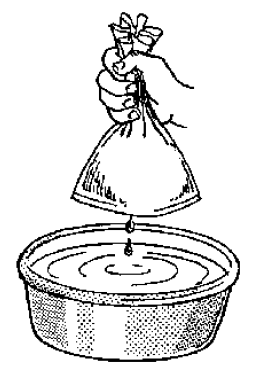
\includegraphics[width=0.4\textwidth]{./img/source/water-waves.png}
\end{center}

\begin{description*}
%\item[Subtopic:]{}
\item[Materials:]{}
\item[Setup:]{}
\item[Procedure:]{}
\item[Hazards:]{}
\item[Questions:]{}
\item[Observations:]{}
\item[Theory:]{}
\item[Applications:]{}
\item[Notes:]{}
\end{description*}

\subsection{Flick-Sticks}

\begin{center}
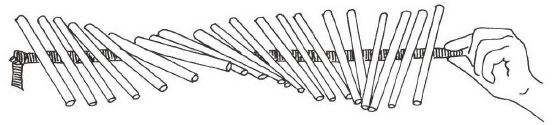
\includegraphics[width=0.4\textwidth]{./img/vso/flick-sticks.png}
\end{center}

\begin{description*}
%\item[Subtopic:]{}
\item[Materials:]{}
\item[Setup:]{}
\item[Procedure:]{}
\item[Hazards:]{}
\item[Questions:]{}
\item[Observations:]{}
\item[Theory:]{}
\item[Applications:]{}
\item[Notes:]{}
\end{description*}

%==================================================================================================%

\section*{Properties of Waves}


\subsection{Water Bottle Sine Wave}

\begin{center}
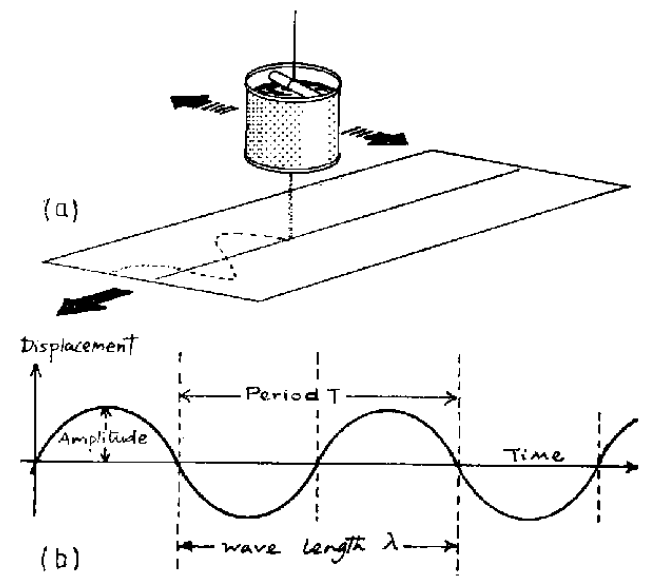
\includegraphics[width=0.4\textwidth]{./img/source/sine-wave.png}
\end{center}

\begin{description*}
%\item[Subtopic:]{}
\item[Materials:]{}
\item[Setup:]{}
\item[Procedure:]{}
\item[Hazards:]{}
\item[Questions:]{}
\item[Observations:]{}
\item[Theory:]{}
\item[Applications:]{}
\item[Notes:]{}
\end{description*}

\subsection{Student Waves}

\begin{center}
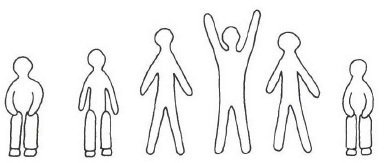
\includegraphics[width=0.4\textwidth]{./img/vso/student-waves.png}
\end{center}

\begin{description*}
%\item[Subtopic:]{}
\item[Materials:]{}
\item[Setup:]{}
\item[Procedure:]{}
\item[Hazards:]{}
\item[Questions:]{}
\item[Observations:]{The wave carries energy as it passes through the students, but each individual student does not travel with the wave.}
\item[Theory:]{}
\item[Applications:]{}
\item[Notes:]{}
\end{description*}

\subsection{Transfer of Energy}

\begin{center}
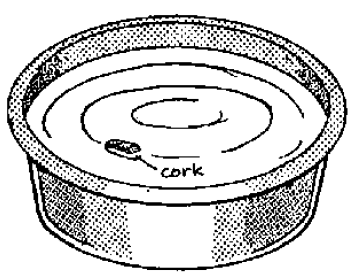
\includegraphics[width=0.4\textwidth]{./img/source/trans-energy.png}
\end{center}

\begin{description*}
%\item[Subtopic:]{}
\item[Materials:]{}
\item[Setup:]{}
\item[Procedure:]{}
\item[Hazards:]{}
\item[Questions:]{}
\item[Observations:]{}
\item[Theory:]{}
\item[Applications:]{}
\item[Notes:]{}
\end{description*}

%==================================================================================================%

\section*{Types of Waves}


\subsection{Slinky Spring}

%\begin{center}
%\includegraphics[width=0.4\textwidth]{./img/source/.png}
%\end{center}

\begin{description*}
%\item[Subtopic:]{}
\item[Materials:]{}
\item[Setup:]{}
\item[Procedure:]{}
\item[Hazards:]{}
\item[Questions:]{}
\item[Observations:]{}
\item[Theory:]{}
\item[Applications:]{}
\item[Notes:]{}
\end{description*}

\subsection{Transverse Pendulum}

\begin{center}
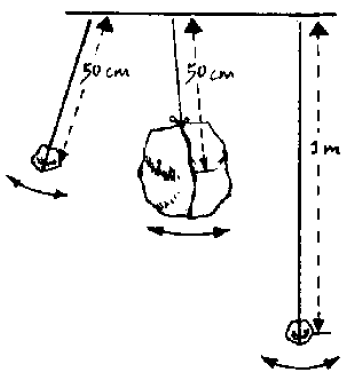
\includegraphics[width=0.4\textwidth]{./img/source/transverse-pendulum.png}
\end{center}

\begin{description*}
%\item[Subtopic:]{}
\item[Materials:]{}
\item[Setup:]{}
\item[Procedure:]{}
\item[Hazards:]{}
\item[Questions:]{}
\item[Observations:]{}
\item[Theory:]{}
\item[Applications:]{}
\item[Notes:]{}
\end{description*}

\subsection{Longitudinal Pendulum}

\begin{center}
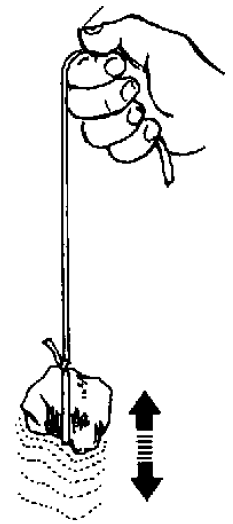
\includegraphics[width=0.4\textwidth]{./img/source/longitudinal-pendulum.png}
\end{center}

\begin{description*}
%\item[Subtopic:]{}
\item[Materials:]{}
\item[Setup:]{}
\item[Procedure:]{}
\item[Hazards:]{}
\item[Questions:]{}
\item[Observations:]{}
\item[Theory:]{}
\item[Applications:]{}
\item[Notes:]{}
\end{description*}

\subsection{Longitudinal Student Waves}

\begin{center}
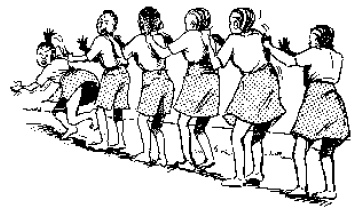
\includegraphics[width=0.4\textwidth]{./img/source/longitudinal-waves.png}
\end{center}

\begin{description*}
%\item[Subtopic:]{}
\item[Materials:]{}
\item[Setup:]{}
\item[Procedure:]{}
\item[Hazards:]{}
\item[Questions:]{}
\item[Observations:]{}
\item[Theory:]{}
\item[Applications:]{}
\item[Notes:]{}
\end{description*}

%==================================================================================================%

\section*{Behaviour of Waves}


\subsection{Construction of a Ripple Tank}

% Different pic???
\begin{center}
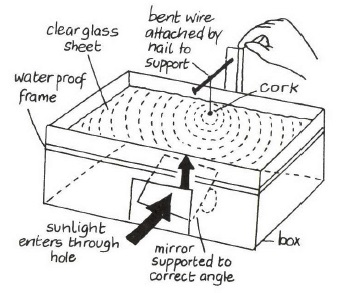
\includegraphics[width=0.4\textwidth]{./img/vso/ripple-tank.png}
\end{center}

\begin{description*}
%\item[Subtopic:]{}
\item[Materials:]{}
\item[Setup:]{}
\item[Procedure:]{}
\item[Hazards:]{}
\item[Questions:]{}
\item[Observations:]{}
\item[Theory:]{}
\item[Applications:]{}
\item[Notes:]{}
\end{description*}

\subsection{Using the Ripple Tank}

%\begin{center}
%\includegraphics[width=0.4\textwidth]{./img/source/.png}
%\end{center}

\begin{description*}
%\item[Subtopic:]{}
\item[Materials:]{}
\item[Setup:]{}
\item[Procedure:]{}
\item[Hazards:]{}
\item[Questions:]{}
\item[Observations:]{}
\item[Theory:]{}
\item[Applications:]{}
\item[Notes:]{}
\end{description*}

%==================================================================================================%

\section*{Reflection of Waves}


\subsection{Reflection of Water Waves}

\begin{center}
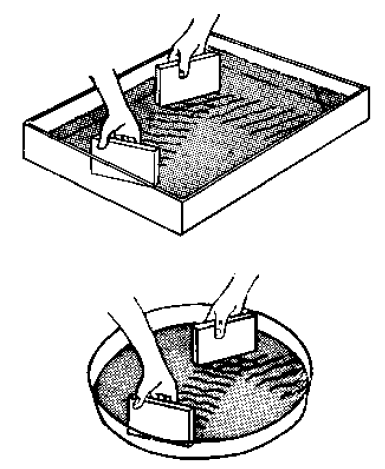
\includegraphics[width=0.4\textwidth]{./img/source/reflection-water-waves.png}
\end{center}

\begin{description*}
%\item[Subtopic:]{}
\item[Materials:]{}
\item[Setup:]{}
\item[Procedure:]{}
\item[Hazards:]{}
\item[Questions:]{}
\item[Observations:]{}
\item[Theory:]{}
\item[Applications:]{}
\item[Notes:]{}
\end{description*}

\subsection{Reflection of Sound Waves}

\begin{center}
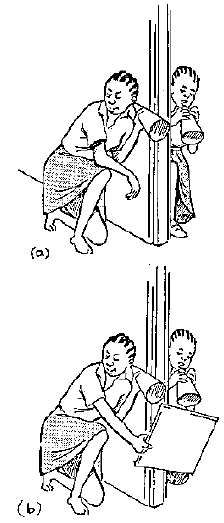
\includegraphics[width=0.4\textwidth]{./img/source/reflection-sound-waves.png}
%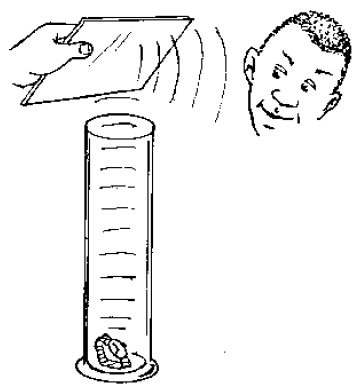
\includegraphics[width=0.4\textwidth]{./img/source/reflection-sound-waves-2.png}
\end{center}

\begin{description*}
%\item[Subtopic:]{}
\item[Materials:]{}
\item[Setup:]{}
\item[Procedure:]{}
\item[Hazards:]{}
\item[Questions:]{}
\item[Observations:]{}
\item[Theory:]{}
\item[Applications:]{}
\item[Notes:]{}
\end{description*}

\subsection{Reflection in a Rope}

\begin{center}
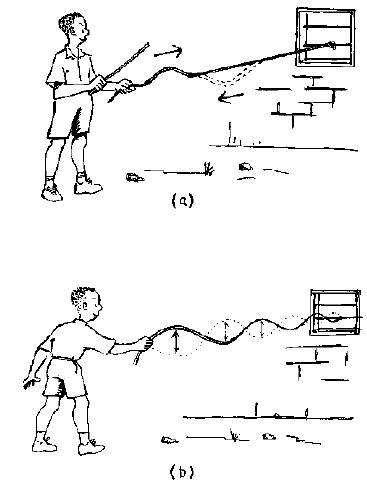
\includegraphics[width=0.4\textwidth]{./img/source/reflection-rope-waves.png}
\end{center}

\begin{description*}
%\item[Subtopic:]{}
\item[Materials:]{}
\item[Setup:]{}
\item[Procedure:]{}
\item[Hazards:]{}
\item[Questions:]{}
\item[Observations:]{}
\item[Theory:]{}
\item[Applications:]{}
\item[Notes:]{}
\end{description*}

\subsection{Reflection in a Hose Pipe}

\begin{center}
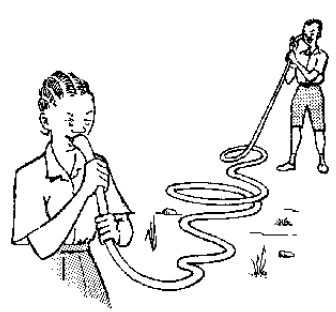
\includegraphics[width=0.4\textwidth]{./img/source/reflection-hose-waves.png}
\end{center}

\begin{description*}
%\item[Subtopic:]{}
\item[Materials:]{}
\item[Setup:]{}
\item[Procedure:]{}
\item[Hazards:]{}
\item[Questions:]{}
\item[Observations:]{}
\item[Theory:]{}
\item[Applications:]{}
\item[Notes:]{}
\end{description*}

%==================================================================================================%

\section*{Sound Waves}


\subsection{Sound from a Ruler}

\begin{center}
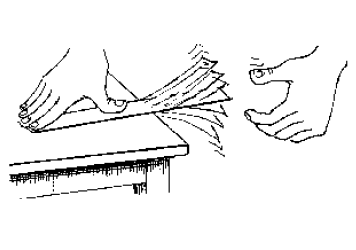
\includegraphics[width=0.4\textwidth]{./img/source/sound-ruler.png}
\end{center}

\begin{description*}
%\item[Subtopic:]{}
\item[Materials:]{}
\item[Setup:]{}
\item[Procedure:]{}
\item[Hazards:]{}
\item[Questions:]{}
\item[Observations:]{}
\item[Theory:]{}
\item[Applications:]{}
\item[Notes:]{}
\end{description*}

\subsection{Straw Kazoo}

%\begin{center}
%\includegraphics[width=0.4\textwidth]{./img/source/.png}
%\end{center}

\begin{description*}
%\item[Subtopic:]{}
\item[Materials:]{}
\item[Setup:]{}
\item[Procedure:]{}
\item[Hazards:]{}
\item[Questions:]{}
\item[Observations:]{}
\item[Theory:]{}
\item[Applications:]{}
\item[Notes:]{}
\end{description*}

\subsection{Sound Sandwich}

\begin{center}
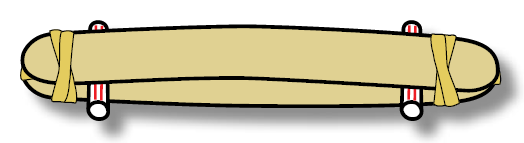
\includegraphics[width=0.4\textwidth]{./img/sound-sandwich.jpg}
\end{center}

\begin{description*}
%\item[Subtopic:]{}
\item[Materials:]{}
\item[Setup:]{}
\item[Procedure:]{}
\item[Hazards:]{}
\item[Questions:]{}
\item[Observations:]{}
\item[Theory:]{}
\item[Applications:]{}
\item[Notes:]{}
\end{description*}

\subsection{Sound Vibrations}

\begin{center}
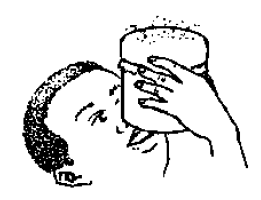
\includegraphics[width=0.4\textwidth]{./img/source/sound-vibrations.png}
\end{center}

\begin{description*}
%\item[Subtopic:]{}
\item[Materials:]{}
\item[Setup:]{}
\item[Procedure:]{}
\item[Hazards:]{}
\item[Questions:]{}
\item[Observations:]{}
\item[Theory:]{}
\item[Applications:]{}
\item[Notes:]{}
\end{description*}

\subsection{Drum Vibrations}

\begin{center}
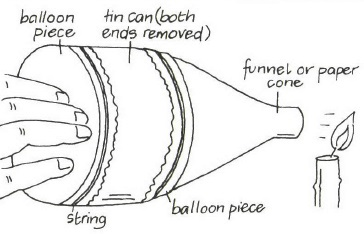
\includegraphics[width=0.4\textwidth]{./img/vso/drum-vibrations.png}
\end{center}

\begin{description*}
%\item[Subtopic:]{}
\item[Materials:]{}
\item[Setup:]{}
\item[Procedure:]{}
\item[Hazards:]{}
\item[Questions:]{}
\item[Observations:]{}
\item[Theory:]{}
\item[Applications:]{}
\item[Notes:]{}
\end{description*}

\subsection{Knocking a Water Tank}

\begin{center}
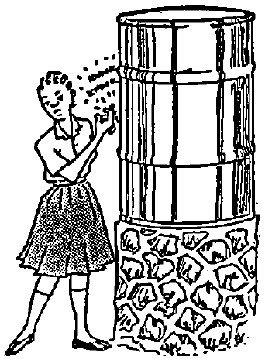
\includegraphics[width=0.4\textwidth]{./img/source/knocking-water-tank.png}
\end{center}

\begin{description*}
%\item[Subtopic:]{}
\item[Materials:]{}
\item[Setup:]{}
\item[Procedure:]{}
\item[Hazards:]{}
\item[Questions:]{}
\item[Observations:]{}
\item[Theory:]{}
\item[Applications:]{}
\item[Notes:]{}
\end{description*}

%==================================================================================================%

\section*{Propagation of Sound Waves}


\subsection{String Telephone}

\begin{center}
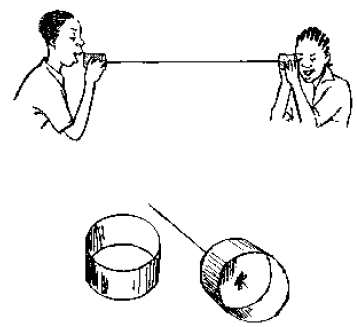
\includegraphics[width=0.4\textwidth]{./img/source/string-telephone.png}
\end{center}

\begin{description*}
%\item[Subtopic:]{}
\item[Materials:]{}
\item[Setup:]{}
\item[Procedure:]{}
\item[Hazards:]{}
\item[Questions:]{}
\item[Observations:]{}
\item[Theory:]{}
\item[Applications:]{}
\item[Notes:]{}
\end{description*}

\subsection{Sound in Air}

\begin{center}
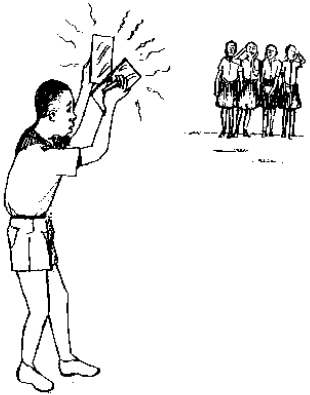
\includegraphics[width=0.4\textwidth]{./img/source/sound-in-air.png}
\end{center}

\begin{description*}
%\item[Subtopic:]{}
\item[Materials:]{}
\item[Setup:]{}
\item[Procedure:]{}
\item[Hazards:]{}
\item[Questions:]{}
\item[Observations:]{}
\item[Theory:]{}
\item[Applications:]{}
\item[Notes:]{}
\end{description*}

\subsection{Sound in a String}

\begin{center}
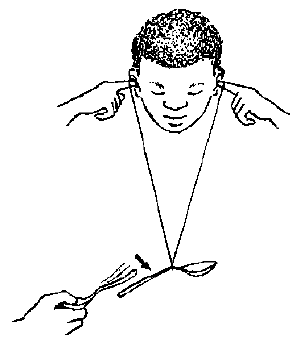
\includegraphics[width=0.4\textwidth]{./img/source/sound-in-string.png}
\end{center}

\begin{description*}
%\item[Subtopic:]{}
\item[Materials:]{}
\item[Setup:]{}
\item[Procedure:]{}
\item[Hazards:]{}
\item[Questions:]{}
\item[Observations:]{}
\item[Theory:]{}
\item[Applications:]{}
\item[Notes:]{}
\end{description*}

\subsection{Sound in Wood}

\begin{center}
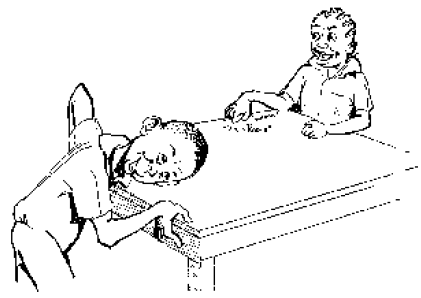
\includegraphics[width=0.4\textwidth]{./img/source/sound-in-wood.png}
\end{center}

\begin{description*}
%\item[Subtopic:]{}
\item[Materials:]{}
\item[Setup:]{}
\item[Procedure:]{}
\item[Hazards:]{}
\item[Questions:]{}
\item[Observations:]{}
\item[Theory:]{}
\item[Applications:]{}
\item[Notes:]{}
\end{description*}

\subsection{Sound in Metal}

\begin{center}
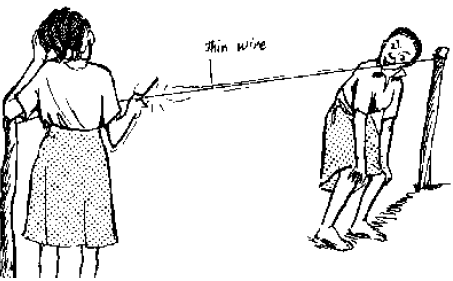
\includegraphics[width=0.4\textwidth]{./img/source/sound-in-metal.png}
\end{center}

\begin{description*}
%\item[Subtopic:]{}
\item[Materials:]{}
\item[Setup:]{}
\item[Procedure:]{}
\item[Hazards:]{}
\item[Questions:]{}
\item[Observations:]{}
\item[Theory:]{}
\item[Applications:]{}
\item[Notes:]{}
\end{description*}

\subsection{Sound in Water}

\begin{center}
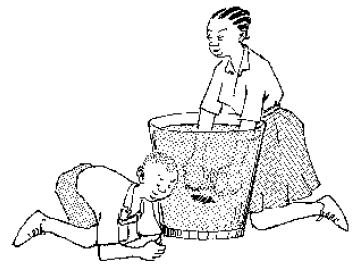
\includegraphics[width=0.4\textwidth]{./img/source/sound-in-water.png}
\end{center}

\begin{description*}
%\item[Subtopic:]{}
\item[Materials:]{}
\item[Setup:]{}
\item[Procedure:]{}
\item[Hazards:]{}
\item[Questions:]{}
\item[Observations:]{}
\item[Theory:]{}
\item[Applications:]{}
\item[Notes:]{}
\end{description*}

\subsection{Doppler Whirl}

%\begin{center}
%\includegraphics[width=0.4\textwidth]{./img/source/.png}
%\end{center}

\begin{description*}
%\item[Subtopic:]{}
\item[Materials:]{}
\item[Setup:]{}
\item[Procedure:]{}
\item[Hazards:]{}
\item[Questions:]{}
\item[Observations:]{}
\item[Theory:]{}
\item[Applications:]{}
\item[Notes:]{}
\end{description*}

%==================================================================================================%

\section*{Musical Instruments}


\subsection{Bottle Orchestra}

\begin{center}
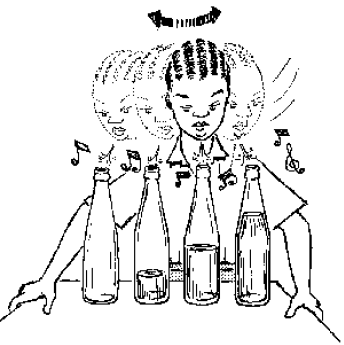
\includegraphics[width=0.4\textwidth]{./img/source/bottle-orchestra.png}
\end{center}

\begin{description*}
%\item[Subtopic:]{}
\item[Materials:]{}
\item[Setup:]{}
\item[Procedure:]{}
\item[Hazards:]{}
\item[Questions:]{}
\item[Observations:]{}
\item[Theory:]{}
\item[Applications:]{}
\item[Notes:]{}
\end{description*}

\subsection{Bamboo Organ}

\begin{center}
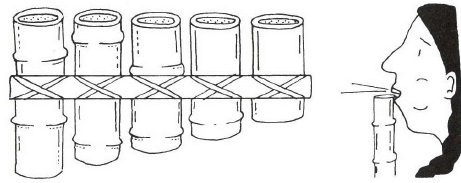
\includegraphics[width=0.4\textwidth]{./img/vso/bamboo-organ.png}
\end{center}

\begin{description*}
%\item[Subtopic:]{}
\item[Materials:]{}
\item[Setup:]{}
\item[Procedure:]{}
\item[Hazards:]{}
\item[Questions:]{}
\item[Observations:]{}
\item[Theory:]{}
\item[Applications:]{}
\item[Notes:]{}
\end{description*}

\subsection{Bamboo Flute}

\begin{center}
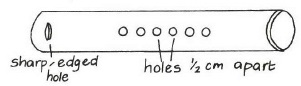
\includegraphics[width=0.4\textwidth]{./img/vso/bamboo-flute.png}
\end{center}

\begin{description*}
%\item[Subtopic:]{}
\item[Materials:]{}
\item[Setup:]{}
\item[Procedure:]{}
\item[Hazards:]{}
\item[Questions:]{}
\item[Observations:]{}
\item[Theory:]{}
\item[Applications:]{}
\item[Notes:]{}
\end{description*}

\subsection{Marimba}

\begin{center}
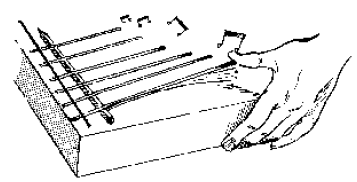
\includegraphics[width=0.4\textwidth]{./img/source/marimba.png}
\end{center}

\begin{description*}
%\item[Subtopic:]{}
\item[Materials:]{}
\item[Setup:]{}
\item[Procedure:]{}
\item[Hazards:]{}
\item[Questions:]{}
\item[Observations:]{}
\item[Theory:]{}
\item[Applications:]{}
\item[Notes:]{}
\end{description*}

\subsection{Xylophone}

\begin{center}
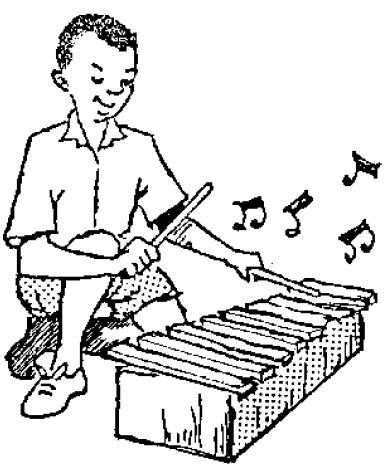
\includegraphics[width=0.4\textwidth]{./img/source/xylophone.png}
\end{center}

\begin{description*}
%\item[Subtopic:]{}
\item[Materials:]{}
\item[Setup:]{}
\item[Procedure:]{}
\item[Hazards:]{}
\item[Questions:]{}
\item[Observations:]{}
\item[Theory:]{}
\item[Applications:]{}
\item[Notes:]{}
\end{description*}

%==================================================================================================%

\section*{Stationary Waves}


\subsection{Sonometer (One-String Guitar)}

\begin{center}
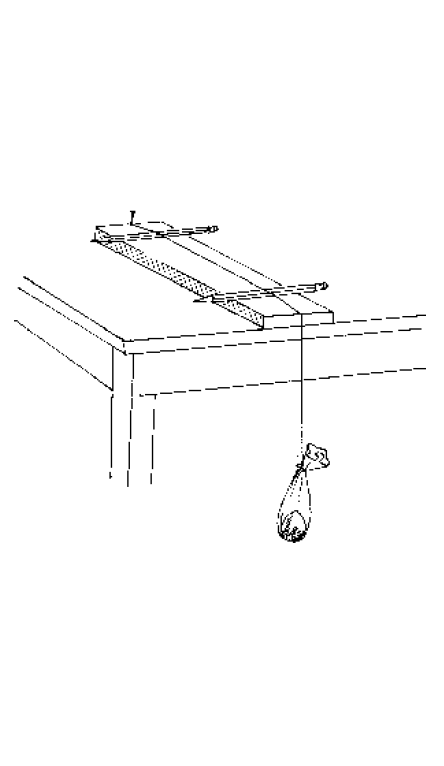
\includegraphics[width=0.4\textwidth]{./img/source/sonometer.png}
\end{center}

\begin{description*}
%\item[Subtopic:]{}
\item[Materials:]{}
\item[Setup:]{}
\item[Procedure:]{}
\item[Hazards:]{}
\item[Questions:]{}
\item[Observations:]{}
\item[Theory:]{}
\item[Applications:]{}
\item[Notes:]{}
\end{description*}

\subsection{Resonance Tube}

\begin{center}
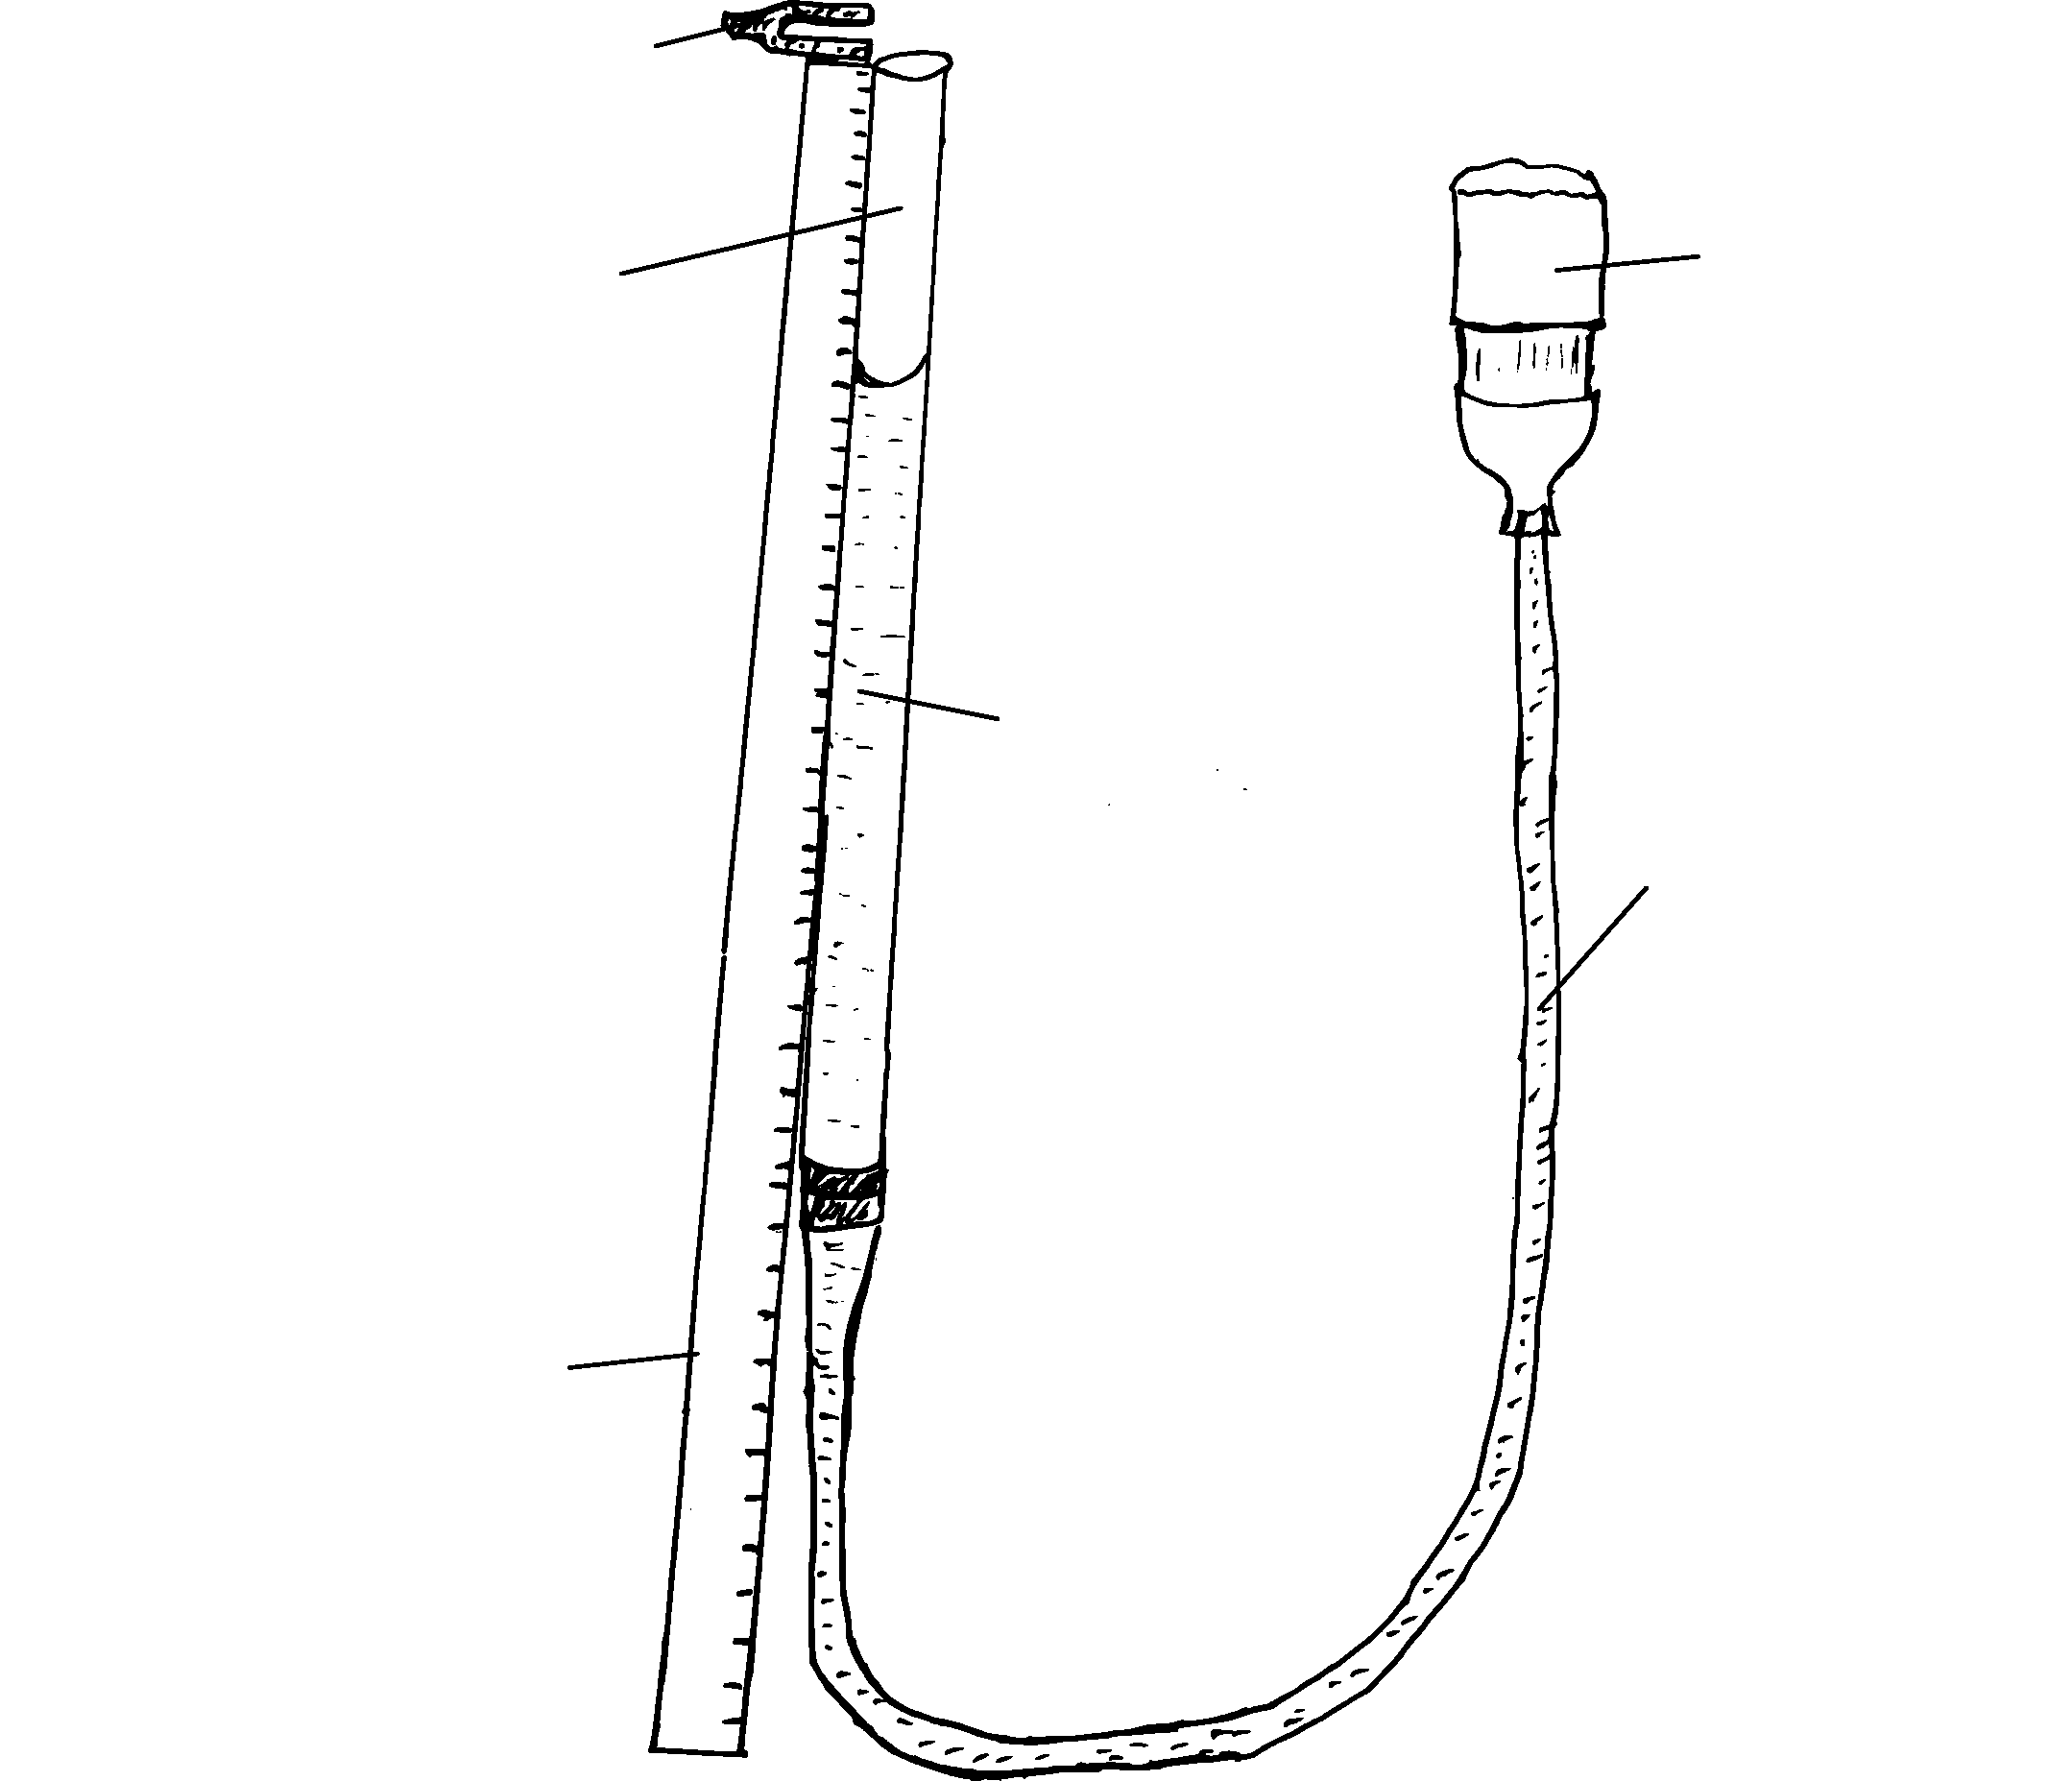
\includegraphics[width=0.4\textwidth]{./img/resonance-tube.png}
\end{center}

\begin{description*}
%\item[Subtopic:]{}
\item[Materials:]{}
\item[Setup:]{}
\item[Procedure:]{}
\item[Hazards:]{}
\item[Questions:]{}
\item[Observations:]{}
\item[Theory:]{}
\item[Applications:]{}
\item[Notes:]{}
\end{description*}

%==================================================================================================%


%\subsection{Speed of Sound in Air}
%
%%\begin{center}
%%\includegraphics[width=0.4\textwidth]{./img/source/.png}
%%\end{center}
%
%\begin{description*}
%%\item[Subtopic:]{}
%\item[Materials:]{}
%\item[Setup:]{}
%\item[Procedure:]{}
%\item[Hazards:]{}
%\item[Questions:]{}
%\item[Observations:]{}
%\item[Theory:]{}
%\item[Applications:]{}
%\item[Notes:]{}
%\end{description*}

\end{multicols}

\pagebreak